% Elsevier numeric-reference template, single-column review manuscript.
\documentclass[review,12pt]{elsarticle}
\biboptions{numbers,sort&compress}
\newenvironment{kbsmalltable}{\begin{table}[htbp]}{\end{table}}
\usepackage{microtype}
\usepackage{amsmath,amssymb,amsthm}
\usepackage{booktabs,graphicx,array,adjustbox,placeins}
\usepackage{xurl,hyperref,enumitem}
\setlength{\emergencystretch}{3em}
\hypersetup{hidelinks,pdftitle={Compact Rule Distillation with Diagnostic Allocation and Certified Feature Forgetting},pdfauthor={Xu Wang and Zhiqiang Chen}}
\journal{Knowledge-Based Systems}
\makeatletter
% Keep float-only pages aligned at the top, with consistent table spacing.
\setlength{\@fptop}{0pt}
\setlength{\@fpsep}{12pt}
\setlength{\@fpbot}{0pt plus 1fil}
\setlength{\@dblfptop}{0pt}
\setlength{\@dblfpsep}{12pt}
\setlength{\@dblfpbot}{0pt plus 1fil}
\makeatother
\newenvironment{kbtable}{\begin{table}[htbp]}{\end{table}}
\newenvironment{kbfigure}{\begin{figure}[htbp]}{\end{figure}}
\newcommand{\kbsbarrier}{\FloatBarrier}
\setcounter{dbltopnumber}{4}
\renewcommand{\dbltopfraction}{0.9}
\renewcommand{\dblfloatpagefraction}{0.6}
\renewcommand{\textfraction}{0.1}
\newtheorem{proposition}{Proposition}
\newcommand{\method}{Diagnostic LFIO}
\newcommand{\evidence}{docs/research/paper_2026-09-24}
\newcommand{\IndependentDiagnosticBF}{89.76}
\newcommand{\IndependentMedianBF}{88.57}
\newcommand{\IndependentMDLBF}{90.77}
\newcommand{\IndependentGain}{+1.19}
\newcommand{\IndependentGainLow}{-0.46}
\newcommand{\IndependentGainHigh}{+2.95}
\newcommand{\IndependentStop}{70.8}
\newcommand{\IndependentWork}{58.7}
\newcommand{\IndependentOptimal}{6}

\newcommand{\GeneralizationSaved}{4.78}
\newcommand{\GeneralizationChange}{-0.017}

\newcommand{\ForgettingCoverage}{80.8}
\newcommand{\ForgettingGain}{+19.8}
\newcommand{\ForgettingPairCoverage}{61.4}

\newcommand{\ContextCost}{27.9}
\newcommand{\ContextCoverage}{89.9}
\newcommand{\ContextGain}{2.0}
\newcommand{\ContextGainLow}{0.9}
\newcommand{\ContextGainHigh}{3.1}
\newcommand{\ContextQueryGained}{51892}

\begin{document}
\begin{frontmatter}
\title{Compact Rule Distillation with Diagnostic Allocation and Certified Feature Forgetting}
\author[1,2,3]{Xu Wang\corref{cor1}}
\ead{xwang@idt.eitech.edu.cn}
\author[1,2,3]{Zhiqiang Chen}
\ead{zqchen@idt.eitech.edu.cn}
\cortext[cor1]{Corresponding author.}
\affiliation[1]{organization={Ningbo Institute of Digital Twin, Eastern Institute of Technology},city={Ningbo},postcode={315200},state={Zhejiang},country={P.R. China}}
\affiliation[2]{organization={Ningbo Key Laboratory of Spatial Intelligence and Digital Derivative},city={Ningbo},postcode={315200},state={Zhejiang},country={P.R. China}}
\affiliation[3]{organization={Zhejiang Key Laboratory of Industrial Intelligence and Digital Twin},city={Ningbo},postcode={315200},state={Zhejiang},country={P.R. China}}
\begin{abstract}
Compact rule surrogates can lose fidelity through their predicate vocabulary, description budget or search, and can still require unavailable or costly inputs. We combine empirical error attribution, fitting-only effort allocation and certified numerical feature forgetting. A partition-decoder floor and finite-pool integer-programming bounds distinguish training restrictions. Diagnostic LFIO probes interventions while respecting the deployment condition and scoring budgets. A prospectively frozen six-dataset study evaluates 72 numerical-teacher settings and 1,728 budget selections across eight methods. The controller attains \IndependentDiagnosticBF\% macro fidelity at the primary endpoint versus \IndependentMedianBF\% for median-vocabulary restarts; stronger fixed MDL predicates limit the adaptive claim. Explicit generalization adds verified equivalent compression and separately calibrated expansion. Feature forgetting then certifies decisions invariant to hidden coordinates, or abstains. The extension supports exact rational difference constraints, rejects infeasible retained inputs, and answers cached residual queries without compiling a global envelope. On 648 known source fits, a selection-coverage-constrained cost policy hides \ContextCost\% of controlled active-feature cost at \ContextCoverage\% test certified coverage, improving hidden cost over coverage-first selection by \ContextGain{} points (descriptive six-dataset interval [\ContextGainLow,\ContextGainHigh]). Residual queries recover \ContextQueryGained{} assigned test-row queries from earlier compiler fallbacks. Classical forgetting identities are explicitly attributed. These source-relative certificates, synthetic costs and reused datasets establish neither teacher correctness nor human comprehension.
\end{abstract}
\begin{keyword}
Rule distillation \sep Error attribution \sep Feature forgetting \sep Background knowledge \sep Certified partial predictions \sep Input costs
\end{keyword}
\end{frontmatter}
\hypersetup{pdfauthor={Xu Wang and Zhiqiang Chen}}

\section{Introduction}
A compact global rule surrogate must reproduce a teacher's decisions while fitting a description that can be inspected~\citep{craven1995,wang2017brs,lawless2023}. When it fails, spending more computation is only one possible response. A coarse numerical encoding may have already erased distinctions made by the teacher; a small rule budget may exclude an accurate program; or the optimizer may have missed an admissible program. These mechanisms require different interventions. Their separation becomes especially relevant under noisy supervision, which changes both the teacher and the targets available for extraction~\citep{frenay2014,raikovskaia2026}.

Recent advances strengthen the need for this attribution. NeuRules jointly learns discretizations and ordered rules~\citep{xu2025}; FastSRS searches sparse DNF models and their Rashomon sets~\citep{molero2026}; recent methods also learn oblique predicates or explicitly optimize rule stability~\citep{behzadimanesh2026,liu2025moss}. A fidelity ranking across different languages cannot by itself identify whether an improvement comes from search, available predicates, or effective capacity. Equal nominal size also leaves differences in executable tests, validation opportunities, and fitting computation.

Our earlier extractor combined pure and ordinary greedy starts with add/delete/replace repair. The development evidence exposes a limit to that approach: repair does not show a reliable advantage over additional greedy restarts when feasible-neighbor scoring work is matched. Moreover, median-bin tasks can collapse to only eight input patterns, and repeatedly splitting the same datasets does not supply independent external evidence. We therefore change the central algorithmic question from adding search components to deciding whether an additional intervention is useful.

An accurately distilled rule set can still depend on unavailable or costly measurements. We therefore also ask which source decisions remain invariant after hiding whole numerical coordinates, how known domain constraints change that answer, and which inputs can be hidden while preserving a specified measured coverage. This deployment question requires explicit completion semantics and failure states in addition to a compact rule syntax.

This article makes four contributions. First, it places vocabulary, finite-language capacity, and search error on a common empirical scale through valid bounds on the same fitting samples, executable language and condition budget. Second, Diagnostic LFIO implements a fitting-only allocation loop with an absolute work allowance; deployment respects the original budget, and its capacity probe is recorded as sensitivity evidence. Third, the numerical postprocessing framework combines verified compression, separately calibrated expansion, and whole-feature forgetting. Its partial-input interface supports exact background difference constraints, distinct infeasibility and uncertainty states, cached residual queries, and cost-aware coordinate selection under a measured coverage requirement. The contribution is this executable, bounded and replayable integration; logical forgetting, quantifier duality and confidence bounds retain their classical attribution. Fourth, separate frozen studies compare recent direct baselines and evaluate the extensions with source locks, choice replay, independent logical oracles and representation costs. The initial six-dataset experiment and subsequent reuse of that cohort remain explicitly distinguished.

The empirical conclusion is qualified. The controller improves the point estimate over median-vocabulary restarts at the primary endpoint, but the interval and stronger fixed-vocabulary controls limit the claim. This is a testable diagnostic and allocation procedure, not evidence of a generally superior rule optimizer. Earlier studies remain separate in the development supplement; their observations are not used to increase the new study's effective sample size.

\section{Related work}
\subsection{Global distillation and explanatory scope}
Extracting an interpretable approximation of a trained predictor has a long history. TREPAN queries a neural network to build a decision-tree approximation~\citep{craven1995}; later model-extraction work uses active sampling to improve global tree surrogates~\citep{bastani2019}. Knowledge distillation also transfers a teacher's behavior to a student, including through softened class probabilities~\citep{hinton2015}. Our setting uses hard teacher labels on observed fitting and validation inputs, a fixed Boolean vocabulary, and an executable global rule program. It therefore studies agreement under a size constraint, without active query generation or transfer of predictive uncertainty.

Rule syntax alone does not determine explanatory scope. Anchors provides conditions that support an individual prediction with high precision under a specified perturbation distribution~\citep{ribeiro2018}. Here every input receives a prediction from the complete program and its default class, so fidelity is evaluated over the held-out test set. The distinction between an interpretable predictor and an approximation of another predictor also matters~\citep{rudin2019}: our surrogate may reproduce a teacher's errors, and teacher agreement is not evidence of correctness or a faithful account of its internal computation.

Logical forgetting preserves consequences over a retained language while eliminating specified symbols~\citep{lin1994forget}; necessary/sufficient-condition duality has established logical foundations~\citep{lin2001conditions}. Formal XAI already studies sufficient, necessary and complete reasons~\citep{darwiche2020reasons}, and recent work finds most-general inflated explanations for tree ensembles~\citep{izza2025general}. Our feature-forgetting extension compiles both decision boundaries for specified missing numerical coordinates of a DNF surrogate. It does not claim a new forgetting theory or optimize minimal instance explanations. Semantic preservation also need not improve representation size or inference cost~\citep{levy1994forget}; both are measured separately. Background-relative necessary/sufficient conditions are established by Doherty and Sza{\l}as~\citep{doherty2024dualforgetting}. Intentional forgetting in knowledge-graph recommendation~\citep{wang2024forgettingkgrs} supplies a task-impact precedent. Recent Horn forgetting studies~\citep{liberatore2024commonsize,liberatore2025onehead} further motivate explicit size accounting. Their single-head restriction means at most one defining rule per propositional head; it differs from our many-body common-class DNF, so its polynomial guarantee does not apply here.

\subsection{Sparse rule sets and rule lists}
RIPPER combines rule induction with pruning to handle noisy examples~\citep{cohen1995}, while RuleFit learns sparse weighted ensembles of rules~\citep{friedman2008}. Bayesian Rule Sets places priors on small collections of short conjunctions in disjunctive normal form~\citep{wang2017brs}, a representation especially close to our single-head classifier. Scalable Bayesian Rule Lists instead optimizes probabilistic ordered lists of pre-mined rules~\citep{yang2017}. Interpretable Decision Sets jointly addresses prediction and description through criteria including rule length, coverage, and overlap~\citep{lakkaraju2016}. Thus compact rule representation and accuracy--complexity tradeoffs are established ideas, rather than contributions unique to Refined LFIO.

These languages resolve prediction differently: an ordered list uses priority, a weighted ensemble combines rule contributions, and a single-head disjunction uses union coverage followed by an opposite default class. A condition count provides an explicit resource measure, but does not equate their expressive capacity or reading effort. Human experiments on model transparency and feature count show why interpretability claims require task-specific evaluation~\citep{poursabzi2021}. Our experiments measure executable size and fidelity; the RIPPER and RuleFit runs use the \texttt{wittgenstein} and \texttt{imodels} implementations~\citep{wittgenstein,imodels}.

\subsection{Discrete optimization and complexity control}
CORELS provides certificates of optimality for regularized rule-list learning~\citep{angelino2018}, and GOSDT develops exact sparse-tree optimization for several predictive objectives~\citep{lin2020}. These approaches make clear that failures of greedy construction need not be limitations of the model language. More directly related to our representation, Boolean rule-set learning via column generation formulates the accuracy--simplicity tradeoff as an integer program and searches an exponential conjunction space~\citep{dash2018,lawless2023}. Its practical formulation uses a Hamming-loss surrogate that can charge overlapping false-positive rules multiple times; our objective counts each misclassified observation once through union coverage. Its extension also supports fairness constraints. Our enumeration of complete supported depth levels followed by bounded local repair is a different, heuristic search strategy; it supplies no comparable global certificate.

Minimum description length selects models by a coding account of the model and data~\citep{rissanen1978}. MaxSynth applies a description-length objective to learning logic programs from noisy data~\citep{hocquette2024}. Our condition-and-body penalty is only a length regularizer: it does not encode feature identities or constitute a complete description-length code. The finite-pool mixed-integer diagnostic in Section~\ref{sec:real-bounds} instead diagnoses search error under exactly our candidate pool, objective, and budget. CORELS, GOSDT, and MaxSynth are methodological alternatives rather than executed comparators. The approximate BRCG-light experiment below does not replace evaluation of an exact column-generation solver, and the diagnostic establishes no superiority over these optimizers.

FastSRS~\citep{molero2026} is a particularly close recent development: it uses theoretical search-space bounds to efficiently generate sparse DNF classifiers, including multi-value conditions, and collections of near-optimal alternatives. Compact disjunctions and efficient search are consequently established research targets. Our question concerns attribution of extraction error through fixed-vocabulary, capacity, validation, and scored-work controls. Our oracle reports bounds on complete supported depth-two pools for the real fitting samples; it does not explore a Rashomon set or certify all possible numerical predicates. The independent extension executes its official optimizer as a direct baseline, preserves multi-value prediction semantics, and charges each atomic threshold test to the common condition budget.

\subsection{Input/output logic learning and neural rules}
Learning from interpretation transition (LFIT) induces normal logic programs from pairs of interpretations linked by an immediate-consequence operator~\citep{inoue2014}. The original Learning from Input and Output (LFIO) framework learns Datalog programs from input/output sets of ground atoms under least-model semantics~\citep{wang2017lfio}. These are distinct learning settings. Modern inductive logic programming additionally studies background knowledge, recursion, and predicate invention~\citep{cropper2022}. The present Refined LFIO is a propositional classification adaptation: complete Boolean observations map to a single class through nonrecursive conjunctions and an explicit default. The original Datalog framework's semantic and algorithmic guarantees do not automatically transfer to this noise-tolerant heuristic.

Differentiable ILP learns explanatory clauses using a differentiable inference procedure~\citep{evans2018}; D-LFIT extends differentiable learning to interpretation transitions, including mislabeled and incomplete observations~\citep{gao2022}. Recent rule learners explore other relaxations: RNS learns selective logical operators and input negation~\citep{wei2026}, TT-Sparse uses differentiable truth-table components and sparse connectivity~\citep{soegeng2026}, and NeuRules jointly learns discretizations, conjunctions, and rule order~\citep{xu2025}. On complete Boolean inputs, a negated equality is already expressible by its complementary value test. Our contribution therefore concerns the fitting and selection procedure, rather than negation itself. Earlier development compared pinned official TT-Sparse and NeuRules implementations on common Boolean inputs. The independent extension additionally executes NeuRules on continuous numerical inputs, retaining learned interval predicates and ordered hard inference. These adapted distillation experiments do not reproduce the papers' native benchmark suites.

\subsection{Label noise and explanation stability}
Label-noise research distinguishes corruption mechanisms and their effects on predictive performance and learned complexity~\citep{frenay2014}. A survey of noise-handling approaches for deep image classification~\citep{algan2021} covers a different domain that also illustrates why a specified noise model is essential. We use symmetric flips as the primary perturbation and class-dependent and feature-dependent flips as sensitivity checks. These synthetic mechanisms do not reproduce natural annotation errors. In distillation, the teacher mediates the perturbation: changed training labels need not produce changed surrogate targets.

Stability is also a learning objective in its own right. SIRUS extracts frequent rules from random forests to obtain compact predictors with structural stability under data perturbations~\citep{benard2021}. Work on interpretation drift under label noise further separates prediction stability from explanation stability~\citep{raikovskaia2026}. We report feature overlap, canonical body overlap, and prediction agreement separately. Refined LFIO does not explicitly optimize stability, and these measurements do not imply a stability guarantee or human comprehension.

MOSS~\citep{liu2025moss} jointly treats sparsity, accuracy, and stability through multi-objective rule-set optimization. This differs from measuring stability after fitting with an error-and-length objective. Its explicit stability objective also means that robustness cannot be inferred merely from a compact model or higher fidelity to a noise-affected teacher. MOSS is not an executed comparator in this study.


\subsection{Recent knowledge-based rule extraction}
Two recent studies in \emph{Knowledge-Based Systems} sharpen the distinction between a small surrogate and a consistent explanation. FI-rules4XAI~\citep{kozielski2025} combines rule induction with XAI-derived feature importance. Its evaluation considers both agreement in predictions and consistency in the attributes used for decisions. Our objective optimizes predictive error and description length, without enforcing teacher-feature alignment. We therefore add a separate permutation-based feature-use diagnostic; it is not a reproduction of their method or a claim that prediction agreement reveals a teacher's internal reasoning.

CORTEX~\citep{kopanja2025} extends cost-sensitive decision trees to multiclass problems using a class-dependent cost matrix and extracts rules from the resulting trees. Its emphasis is the cost of classification errors and compact extraction across classes. Our setting is binary distillation with an explicit global condition ceiling and an opposite-default disjunction. Class-balanced error weights in our objective do not implement CORTEX's application-specific cost matrix. The studies are complementary in scope; neither CORTEX nor FI-rules4XAI is an executed comparator here. The implemented direct Boolean comparator is the pinned AIX360 BRCG-light variant, whose approximate column-generation search is distinguished from an exact optimization solver.

\subsection{Recent extraction and predicate learning}
Liu et al.~\citep{liu2026extraction} jointly control rule count and interaction depth when extracting regression models from tree ensembles, with exact and approximate optimization and statistical oracle bounds. Their weighted regression rules and access to ensemble structure differ from our hard-label, single-head Boolean distillation. Their results underscore the importance of reporting both structural restrictions and the optimization target; our small-instance objective certificates are not statistical oracle inequalities.

Sparse oblique rule boosting~\citep{behzadimanesh2026} learns sparse linear propositions within additive rule ensembles. It addresses limitations of axis-aligned predicates by changing the condition language. We retain univariate threshold tests and measure the information lost in their encoding; a linear combination involving several inputs cannot be counted as one equivalent Boolean test. Spectral distillation of tree ensembles~\citep{vu2026} instead compresses predictive representations. Compact storage alone does not supply an executable Boolean explanation. These recent alternatives motivate our explicit separation of vocabulary, language capacity, and search, and are not executed comparisons.

\section{Empirical error attribution}\label{sec:diagnostics}
\subsection{Executable language and objectives}
Let $t(x)\in\{0,1\}$ be a fixed teacher and $V=\{x_j>\theta\}$ a numerical predicate vocabulary. Its Boolean encoding is $z_V(x)$. A program $P$ is a set of conjunctions with a common head $h$ and opposite default $1-h$:
\begin{equation}
 f_{P,h}(x)=\begin{cases}h,&\text{some body in }P\text{ is true},\\1-h,&\text{otherwise}.\end{cases}
\end{equation}
A body uses complementary Boolean value tests on distinct encoded features. The description size $s(P)$ is the total number of atomic tests across bodies, including repeated tests in different bodies. The empty program represents a constant. Every deployed model must satisfy $s(P)\leq B$.

We enumerate every conjunction through depth two whose fitting support is at least three, including both values of every predicate. The enumeration ceiling is 75,000 surface candidates; complete depth levels are used. For every vocabulary realized in the independent study the requested levels are admitted. The resulting pool $\mathcal C_V$ is independent of validation and test labels. The fitting class $\mathcal H_{V,B}$ consists of both heads and subsets of this pool with at most 32 bodies and $B$ tests. This is a restricted class: depth, support and the body count are part of its definition.

For a fitting sample with both teacher classes present, set $w_i=1/(2n_{y_i})$, where $y_i=t(x_i)$ and $n_c$ counts class $c$. The balanced training error and search objective are
\begin{align}
 E(P)&=\sum_i w_i\mathbf1[f_{P,h}(x_i)\ne y_i],\\
 J_\alpha(P)&=nE(P)+\alpha\log_2(\max(2,n))\{s(P)+|P|\}.\label{eq:objective}
\end{align}
Union coverage counts each misclassified observation once. The search uses penalties $\alpha\in\{0,0.05,0.2\}$ and both heads; each of these six cells submits its best training-objective program to outer validation. The selected program maximizes validation macro fidelity, then minimizes tests and bodies. Further ties use a fixed penalty/head order. Single-class targets use the exact constant branch and ordinary agreement.

\subsection{A vocabulary floor and bounded decomposition}\label{sec:vocabulary-ceiling}
Group fitting observations by their encoding. Let
\[
 W_{zc}=\sum_{i:z_V(x_i)=z,y_i=c}w_i.
\]
An unrestricted deterministic decoder of this encoding has minimum empirical balanced error
\begin{equation}
 C_V=\sum_z\min(W_{z0},W_{z1}).\label{eq:collision}
\end{equation}
Choosing the lower-error class independently in every group attains this value. With ordinary uniform weights, the corresponding fidelity ceiling is $1-n^{-1}\sum_z\min(n_{z0},n_{z1})$. This identity is a finite-sample partition diagnostic, not a new statistical theorem or a population guarantee. Refining a nested vocabulary cannot increase $C_V$ on the same sample, because each group is subdivided. It can nevertheless worsen small-model generalization or fitting cost.

Let $E^*_{V,B}=\min_{f\in\mathcal H_{V,B}} E(f)$ and let $E_H$ denote any feasible fitted program's error. There is an exact training-sample identity
\begin{equation}
 E_H=C_V+\underbrace{(E^*_{V,B}-C_V)}_{\text{finite-language capacity}}+
                \underbrace{(E_H-E^*_{V,B})}_{\text{search shortfall}}.\label{eq:decomposition}
\end{equation}
Capacity here includes the chosen depth, support and body restrictions, not only the number of conditions. Validation and generalization error are outside this identity.

\begin{proposition}[Finite-pool attribution intervals]\label{prop:intervals}
Suppose a solver gives a valid lower bound $L$ and an incumbent upper bound $U$ for the same error objective over $\mathcal H_{V,B}$. Replace $L$ by $\max(L,C_V)$ and $U$ by $\min(U,E_H)$. Then
\begin{align}
 E^*_{V,B}-C_V&\in[L-C_V,U-C_V],\\
 E_H-E^*_{V,B}&\in[E_H-U,E_H-L].\label{eq:intervals}
\end{align}
The intervals remain valid when the solver times out with a valid dual bound. A zero lower endpoint does not establish that the corresponding mechanism is absent.
\end{proposition}
\begin{proof}
Every feasible rule program is a deterministic decoder of the same encoding, so $C_V\leq E^*_{V,B}$. The solver and feasible-program inequalities give $L\leq E^*_{V,B}\leq U\leq E_H$. Subtracting $C_V$ or reversing the inequalities after subtraction from $E_H$ yields the two intervals. The bounds are coupled through the same unknown optimum; their endpoints cannot be combined arbitrarily as independent component estimates.
\end{proof}

\subsection{Real-task integer-programming bounds}\label{sec:real-bounds}
For each candidate body introduce a binary selection variable. Each distinct observed encoding has an OR-coverage variable constrained to equal the union of the selected covering bodies. Class multiplicities preserve all original observations and their balanced weights. Linear body-count and total-test constraints encode the same feasible class as the heuristic. The oracle minimizes $nE$ without the length penalty, and its reported objective and dual bound are divided by $n$.

We solve both heads separately. The minimum of their valid lower bounds lower-bounds the optimum over both heads; the best solver incumbent or heuristic program supplies an upper bound. The independent protocol fixes six real tasks, clean RF teachers, seed 6001, $B=8$, and both median and median-plus-MDL languages, for 12 class comparisons and 24 head solves. Each solve has a 15-second optimization allowance. Matrix construction and solver overhead are included in reported diagnostic runtime and can exceed that allowance. No fitting rows are subsampled to manufacture a small Boolean task. Only proven optima are called optimal. The older five-bit and parity constructions are retained as supplementary controls rather than substitutes for this real-task analysis.

\section{Fitting-only effort allocation}\label{sec:controller}
\subsection{Absolute work and predicate construction}
The fitting engine uses cached integer coverage, deterministic greedy construction, randomized greedy restarts, and backward deletion. Randomized additions choose uniformly among the three best improving feasible proposals. Training-only selection retains the best program encountered in each cell, with shorter programs breaking objective ties. Every feasible add, delete, or replacement objective score consumes one unit. Fixed repair is a comparator that spends part of the same allowance on bounded add/delete/one-for-one replacement. The controller's default engine uses restarts, reflecting the inconclusive development evidence for repair.

Each budget fit receives at most $W=1{,}200{,}000$ scored-neighbor evaluations, independent of the vocabulary size. A six-cell fit divides its allowance equally, up to integer rounding. This corrects the earlier pool-size-multiplier comparison, whose absolute allocation grew with the number of predicates. Equal scoring ceilings control one defined resource; scoring different-size integers, enumeration, and bookkeeping still have different CPU costs. We report actual scores, CPU and wall time separately.

The median vocabulary has one fitting median per raw feature. Its enriched version retains that median and adds at most two cuts accepted by the established Fayyad--Irani MDL criterion~\citep{fayyad1993}, with minimum leaf support three and best-first truncation. Neither the MDL criterion nor greedy restarts is claimed as a new primitive. All thresholds are learned from the relevant fitting partition and its teacher outputs. Test or outer-validation observations do not determine the vocabulary.

\subsection{Internal action witnesses}
Diagnostic LFIO uses one fitting-internal, group-stratified four-fold split, approximately 75\% for probe fitting and 25\% for probe selection. Identical raw observations stay together. Four probes use the same six penalty/head cells:
\begin{enumerate}[leftmargin=*,itemsep=2pt]
\item \emph{Stop reference}: median predicates, original $B$, allowance $W/24$.
\item \emph{Search}: median predicates, original $B$, allowance $3W/24$.
\item \emph{Vocabulary}: MDL-enriched predicates, original $B$, allowance $W/24$.
\item \emph{Capacity witness}: median predicates, $2B$, allowance $W/24$.
\end{enumerate}
Thus the capacity witness changes only the description allowance relative to its reference, and the vocabulary witness changes the predicates at the same score cap. The search intervention explicitly buys additional scoring work. The six-cell winner of each probe is selected on the internal holdout. These are action experiments on fitting data, distinct from the oracle's certificates.

For an action $a$, let $\widehat\Delta_a$ be its paired macro-fidelity gain over the reference. Within each teacher class, the per-observation change takes values $-1,0,1$. Its within-class sampling variance gives the descriptive standard error
\begin{equation}
 \widehat\sigma_a=\frac12\sqrt{\frac{s_{a0}^2}{n_0}+\frac{s_{a1}^2}{n_1}}.
\end{equation}
The allocation score is $q_a=\widehat\Delta_a-\widehat\sigma_a$. The controller chooses the higher of search and vocabulary only if its score exceeds 0.01; otherwise it stops. This one-standard-error rule is a fixed allocation heuristic, not a confidence bound after probe selection. A capacity score above 0.01 is recorded as a budget-sensitivity witness and cannot authorize an over-budget deployment. Insufficient class/group support skips the probes and selects stop.

\subsection{Final fit and information boundaries}
The selected vocabulary is reconstructed on the complete outer fitting sample. Search and vocabulary actions can spend the remaining scoring allowance; stop restricts the final fit to $W/6$, deliberately saving work. The original condition budget $B$ always applies. Probe work counts toward $W$, and each final cell contributes one program to outer validation. Neither an alternative language nor the double-budget probe is submitted as an additional outer-validation option. Outer validation selects only the six final penalty/head cells. Only after that decision is persisted does the experiment evaluate the exported program on test inputs.

The controller does not use the retrospective test ceiling or the integer-programming certificate to select an action. The former would leak the evaluation target, while the latter can be costly and inconclusive. Its operational signals are fitting-only held-out interventions. The certificate separately assesses whether the vocabulary/capacity/search interpretation is justified on a defined sample and language. In high dimensions, singleton encodings can make $C_V=0$ even when the selected student performs poorly; the action probes remain executable in this case, and the floor is reported as uninformative rather than evidence of adequate predicates.

\section{Explicit generalization of rule surrogates}\label{sec:generalization}
\subsection{Numerical semantics and lossless compression}
The preceding extractor selects short clauses directly; it does not perform a separate literal-deletion or clause-merging generalization pass. We add a post-fitting module for that purpose. Its input is a single-head DNF on finite numerical thresholds, with the same opposite default. A body denotes an axis-aligned box: each coordinate has an exclusive lower bound and an inclusive upper bound. Combining tests on the same raw feature therefore retains only the strongest lower and upper bounds; contradictory bodies disappear.

The exact stage attempts to delete a condition, remove an already covered body, or merge two bodies into their smallest axis-aligned enclosing box. Every proposed whole-program change must pass a global equivalence check. The verifier subtracts the covering boxes from each proposed head region in both directions. An empty residual proves containment; a nonempty residual is a counterexample region. The interval endpoints preserve strict comparisons, including their boundary values. A proof permits at most 20,000 box subtractions and one exact pass permits 500,000. Exhaustion returns \emph{unknown}, which never authorizes a change. Accepted changes strictly reduce the lexicographic count of tests, bodies, raw features and distinct thresholds.

This certificate covers all real inputs under the stated threshold semantics, hence all supported finite float64 inputs, rather than only recorded examples. It preserves agreement with any fixed teacher wherever the original surrogate agreed, but does not establish correctness of that teacher or reveal its internal computation. The greedy result need not be a globally shortest equivalent DNF. Boolean absorption, complementary merging and logical generalization are established operations~\citep{nienhuys1996}; the contribution here is their explicit numerical semantics, bounded whole-program verification and integration with controlled approximate generalization.

\subsection{A grow-only expansion path}
Approximate generalization additionally permits changes that enlarge the head region. Condition deletion and enclosing-box merging provide such changes; subsequent exact compression preserves that enlargement. Let $P_0$ be the original program and $P_j$ a path candidate. For either head $h$, the invariant is
\begin{equation}
 \{x:f_{P_0}(x)=h\}\subseteq\{x:f_{P_j}(x)=h\}.
\end{equation}
Thus a harmful new prediction can occur only when the teacher outputs $1-h$. Writing $f_j=f_{P_j}$, define its conditional rate as
\begin{equation}
 H_j=\Pr\{f_0(X)=1-h,\ f_j(X)=h\mid T(X)=1-h\}.
\end{equation}
For a population with both teacher classes, the two-class balanced-error increase obeys
\begin{equation}\label{eq:generalization-harm}
 E_{\rm bal}(P_j)-E_{\rm bal}(P_0)\leq H_j/2.
\end{equation}
The other teacher class cannot acquire errors under the containment invariant. This elementary one-sided relation does not equate predictive generalization with logical generalization.

The path is built only on grow data. We require cumulative empirical harm at most $2\epsilon$ relative to $P_0$, with $\epsilon=0.02$, rather than resetting the allowance at every move. Among feasible complexity-reducing proposals, the algorithm chooses the shortest lexicographic description, then lower harm and a fixed fingerprint. Each step verifies containment. The full path, including its length $K$, is fixed before calibration. The no-calibration ablation deploys its shortest endpoint.

\subsection{Independent calibration and scope of its bound}
The bounded variant uses a separate calibration partition, excluded from base-model selection and path construction. For candidate $j$, let $k_j$ of $n$ calibration observations from the opposite teacher class incur harmful changes. A one-sided Clopper--Pearson limit~\citep{clopper1934} is
\begin{equation}
 U_j=\operatorname{Beta}^{-1}(1-\delta/K;k_j+1,n-k_j),
\end{equation}
with $U_j=1$ for $n=0$ or $k_j=n$ and $\delta=0.05$. We select the smallest candidate satisfying $U_j/2\leq\epsilon$, or retain the exact model if none qualifies. A second ablation replaces this bound by $k_j/(2n)$; it enforces an observed calibration constraint only.

Conditional on a fixed learner/path and independent iid class-conditional calibration observations, binomial coverage and a union bound yield simultaneous validity for all $K$ candidates with probability at least $1-\delta$. Equation~\ref{eq:generalization-harm} then bounds the selected program's balanced-error increase by $\epsilon$. This is a per-path guarantee, not joint coverage over all study fits, nor a deterministic bound on a finite test fold. The guarantee depends on the sampling assumptions: duplicate-group benchmark splitting alone does not establish population iid sampling. It also does not cover distribution shift or observed-class macro scoring on a single-class test partition. The exact fallback retains its global equivalence guarantee without these probabilistic assumptions.

The public \texttt{GeneralizedLFIO} wrapper exposes exact and calibrated deployment modes, rejects overlapping raw rows across fitting/selection/calibration partitions, exports both programs and proofs, and provides executable prediction traces. Trace readability and structural compression remain proxies rather than measured human comprehension.

\section{Forgetting numerical features}\label{sec:feature-forgetting}
\subsection{Necessary and sufficient conditions on retained inputs}
Deleting one test from one body does not in general eliminate its raw feature from the program. We separately implement whole-coordinate forgetting. Let $F(r,s)$ be the source surrogate's head-region formula, with retained coordinates $r$ and forgotten coordinates $s$. Define
\begin{equation}\label{eq:forgetting-envelope}
 U_S(r)=\exists s\,F(r,s),\qquad
 L_S(r)=\neg\exists s\,\neg F(r,s).
\end{equation}
Both formulas omit every coordinate in $S$, and
\begin{equation}\label{eq:forgetting-sandwich}
 L_S(r)\Rightarrow F(r,s)\Rightarrow U_S(r)
 \quad\text{for every completion }s.
\end{equation}
With unrestricted finite real completions, $U_S$ is the strongest necessary condition and $L_S$ the weakest sufficient condition expressible over the retained coordinates. Existential forgetting and this duality are classical~\citep{lin1994forget,lin2001conditions}. We contribute their numerical implementation and integration, rather than new quantifier identities.

The partial-input predictor returns head $h$ when $L_S$ holds and default $1-h$ when $U_S$ is false. Otherwise it abstains. If both projections are exact, the remaining region admits completions producing either class. This is a deterministic statement about the chosen surrogate. It needs no sampling assumption, but does not certify the teacher's response, a reference label or a causal effect. Applied after bounded generalization, it certifies that generalized surrogate; it does not silently inherit exact agreement with the original surrogate.

\subsection{Numerical construction and bounded failure}
We normalize every body to nonempty intervals before projection. Existential projection then removes all bounds on $S$ in every body: projection distributes over the union of boxes. Normalization order matters: a body containing both $x>2$ and $x\leq1$ remains impossible after forgetting $x$, rather than becoming true. Threshold atoms on one feature are consequently never treated as independent propositions.

The universal formula is constructed by complementing the head union through interval subtraction, projecting the complement, then complementing again. The retained tests remain executable numerical thresholds with exclusive lower and inclusive upper endpoints. The compiler allows 50,000 subtractions and 4,096 intermediate boxes. If either limit is exhausted, it retains exact $U_S$ and substitutes the sound lower formula $L_S=\bot$, explicitly marking universal completion as unresolved. It never labels this fallback an exact ambiguity region. Saved source formulas, construction traces, limits and output fingerprints permit deterministic replay.

Quantification ranges over all finite real values, including values outside observed data ranges. Input rows use float64, but completion certificates concern the wider real domain; an existential region need not contain a representable float64 value at extreme thresholds. We impose no empirical-range restriction or cross-feature feasibility relation. Accordingly, a counterexample completion can lie off the data manifold. Additional domain constraints would define a different forgetting problem.

\subsection{Queries, explanations and representation cost}
The interface accepts NaN in forgotten columns, or only the ordered retained columns; hidden values are never consulted. It exports necessary/sufficient formulas and, on request, symbolic completion boxes for the head and default classes. For example,
\begin{equation}
 F=(x>0\land y>0)\lor(x\leq0\land z>0)
\end{equation}
yields $U_{\{x\}}=(y>0)\lor(z>0)$ and $L_{\{x\}}=(y>0)\land(z>0)$. Both-positive retained values certify the head, both-nonpositive values certify the default, and mixed signs require knowledge of $x$.

Forgetting need not shorten a DNF: complement construction can expand its representation. We therefore count conditions in both explicit formulas and measure runtime and unresolved compilations, following the distinction between semantic preservation and easier reasoning raised by Levy~\citep{levy1994forget}. For a fixed missing-feature set, retained values that certify a class satisfy a sufficient-reason property. We do not search for subset-minimal reasons or maximum-volume inflated explanations, unlike dedicated formal-explanation methods~\citep{darwiche2020reasons,izza2025general}. The policy below selects missing coordinates for coverage; it does not certify that the retained set is a smallest explanation.

\subsection{Background-constrained partial-input certificates}\label{sec:contextual-forgetting}
The unrestricted construction above can admit completions that violate known definitions. For an explicitly supplied background theory $C(r,s)$, define
\begin{align}
 V_C(r)&=\exists s\,C(r,s),\\
 U_C(r)&=\exists s\,[C(r,s)\land F(r,s)],\\
 L_C(r)&=V_C(r)\land\neg\exists s\,[C(r,s)\land\neg F(r,s)].
\end{align}
On feasible retained inputs, these are the familiar necessary/sufficient conditions relative to background knowledge~\citep{doherty2024dualforgetting}. We explicitly require $V_C$: an input with no legal completion must be rejected rather than receiving a vacuous head certificate.

\begin{proposition}[Conditional partial-input certificate]
If $C(r,\cdot)\land F(r,\cdot)$ is satisfiable and $C(r,\cdot)\land\neg F(r,\cdot)$ is unsatisfiable, every legal completion predicts the head. Reversing the tests certifies the default. If both are satisfiable, the input admits opposite predictions; if neither is satisfiable, it is infeasible.
\end{proposition}
\noindent\emph{Proof.} A satisfiable side supplies a legal completion. Unsatisfiability of the opposite side excludes every legal completion of the other class. The two remaining cases follow by the same partition of $C$ into $C\land F$ and $C\land\neg F$. This is the standard semantic argument, not a new forgetting theorem.

The implemented background language is a conjunction of rational difference bounds $x_i-x_j\leq c$ or $x_i-x_j<c$, with a constant-zero node. Equality uses two opposite bounds. An exact Bellman--Ford procedure over rational/infinitesimal pairs rejects negative cycles, including zero cycles containing strict inequalities. A satisfying symbolic potential is converted into rational values with a sufficiently small positive rational infinitesimal, and every returned witness is checked exactly. Input binary64 values and thresholds denote their exact rational values. Thus strict boundaries are not decided by floating-point tolerances. The language covers equality, order, difference bands and individual bounds; it does not cover arbitrary linear combinations or Boolean background theories.

The head query tries compatible DNF bodies. The default query branches over an atom violated in each compatible body and checks the resulting difference constraints. A 50,000-operation allowance yields explicit UNKNOWN on exhaustion. A class is assigned only with a SAT witness and an opposite UNSAT proof; UNKNOWN remains unresolved. Constraints are supplied by the caller, with no inference from observed correlations. Wrong constraints can produce incorrect predictions relative to the true domain even when the conditional logical result is valid.

\subsection{Residual queries and input-cost selection}\label{sec:cost-forgetting}
Global envelopes serve repeated deployment with a fixed missing-coordinate set, but their DNF can expand. The second interface substitutes only retained values, shares identical residual hidden-coordinate DNFs, and checks head/default completion existence directly. Without background constraints it uses bounded interval subtraction for the residual default query. With constraints its cache key additionally includes retained numerical values appearing in $C$, so different feasible regions cannot be conflated merely because their threshold truth values match. The cache holds at most 4,096 entries with least-recently-used eviction. It stores exact hidden-coordinate witnesses; it does not materialize a readable global formula. Sharing and representation accounting are motivated by knowledge compilation~\citep{zeyen2026divkc,liberatore2024commonsize}; no Horn complexity bound is transferred to this numerical DNF language.

For active source features $A$, positive costs $c_j$ and selection inputs $D_{\rm sel}$, the operational objective is
\begin{equation}
 \max_{S\subseteq A}\sum_{j\in S}c_j\quad\text{subject to}\quad
 \widehat{\operatorname{cov}}_{D_{\rm sel}}(S)\geq q,
\end{equation}
under the query work/cache limits and a 512-candidate subset allowance. Coverage counts only certified assignments. The empty subset is a valid fallback; unused coordinates earn no reward. We use greedy heuristics rather than claim subset optimality. Fixed index, source-frequency, singleton-impact and next-coverage policies provide controls. CostAware adds the feasible coordinate minimizing marginal selection-coverage loss per unit cost, breaking ties by larger cost, higher coverage and then index. All choices are saved before test inference.

Wang and Brewster~\citep{wang2024forgettingkgrs} study intentional forgetting of knowledge-graph triples and rule optimization for recommendation, using least-model impact and graph-importance scores. That work motivates task-dependent impact here. Our singleton impact is measured selection uncertainty, and costs are explicit inputs; graph-centrality heuristics are not logical certificates. The present guarantee concerns all numerical completions under the stated constraints, rather than rule firing on one fixed knowledge graph. Neither the greedy objective nor the logical bounds establish minimal human explanations~\citep{calautti2025globalnecessary}.


\section{Independent evaluation protocol}\label{sec:independent-protocol}
\subsection{Unseen datasets and native teachers}
\begin{kbtable}
\centering
\caption{Independent numerical tasks and teacher reference-label balanced accuracy (percent). Each teacher cell averages three fixed splits. Study/Run identifiers are removed from Climate. Rice and Raisin share a morphological domain.}
\label{tab:independent-data}
\small
\begin{adjustbox}{max width=\linewidth}
\begin{tabular}{lrrrrrrr}
\toprule
Dataset & $n$ & $d$ & Class 1 (\%) & RF clean & HGB clean & RF noisy & HGB noisy \\
\midrule
Rice & 3810 & 7 & 42.8 & 92.71 & 92.07 & 89.51 & 86.55 \\
Raisin & 900 & 7 & 50.0 & 85.19 & 86.30 & 79.44 & 75.19 \\
HTRU2 & 17898 & 8 & 9.2 & 92.06 & 93.67 & 91.59 & 91.28 \\
QSAR & 1055 & 41 & 33.7 & 82.56 & 82.43 & 77.37 & 72.84 \\
Climate & 540 & 18 & 91.5 & 62.96 & 83.67 & 60.61 & 67.34 \\
Retinopathy & 1151 & 19 & 53.1 & 71.10 & 70.48 & 67.74 & 64.05 \\
\bottomrule
\end{tabular}
\end{adjustbox}
\end{kbtable}

The new cohort contains UCI Rice, Raisin, HTRU2, QSAR biodegradation, Climate Model Simulation Crashes, and Diabetic Retinopathy Debrecen~\citep{rice2019,raisin2020,htru2015,qsar2013,climate2013,retinopathy2014}. They were not part of the preceding ten-dataset development work. Their source pages, CC BY 4.0 licenses, raw archives and hashes are recorded with the release. Rice and Raisin concern related morphological measurements; six datasets should not be interpreted as six entirely unrelated application domains. Climate Study/Run identifiers are excluded. We use all rows and the numerical predictors, with binary targets defined in the recorded loaders.

For each dataset, seeds 6001--6003 give group-stratified 60/20/20 fitting/validation/test partitions; exact raw duplicates cannot cross partitions. Two teachers fit native numerical features: a 300-tree RF with minimum leaf support two and balanced-subsample class weights, and HGB with 150 boosting iterations, 31 leaves, L2 penalty one and balanced class weights. Clean or independently 20\%-flipped reference labels supervise the teacher's fitting fold only. Teachers and surrogates receive no corrupted test reference labels. Distillation uses the teacher's hard outputs, including its errors, on the appropriate partitions. The full cross-product is 72 teacher settings.

The protocol and source/data fingerprints were saved before the first model fit in this cohort. This is a same-session prospective freeze after inspecting development results, not an external registry preregistration. We did not adjust its switching threshold, search allowance or vocabulary after seeing independent test outcomes. Ordinary fidelity and reference-label performance are reported alongside macro fidelity to expose class imbalance and teacher quality.

\subsection{Fixed policies and direct baselines}
Condition ceilings are 8/16/32. Fixed median restarts, fixed MDL restarts, and fixed median repair receive the same maximum $W$ per ceiling as Diagnostic LFIO, without spending work on probes. All use the same depth, penalty/head grid, support and body cap. A shared maximum does not force identical actual use; the controller can stop early. These are policy controls, not independent claims of novel rule learners.

The directly executed classical baselines are a native numerical tree, AIX360 BRCG-light~\citep{dash2018,lawless2023}, and official FastSRS~\citep{molero2026}. Trees use maximum leaf counts 2/3/4/6/8/16 and minimum leaf support three. Their predictions are exported as the shorter-head, exactly equivalent single-head DNF, preserving sklearn's float32 input semantics. BRCG-light and FastSRS receive the same fitting-only MDL predicates as the fixed enriched control. Each uses three penalties $0.0005/0.005/0.05$ and both heads. BRCG-light uses depth three, 25 column-generation iterations, its bounded beam pricing/rounding, CLARABEL and a ten-second internal limit; it is not an exact branch-and-price solver.

FastSRS is pinned to official commit \texttt{594904e}, with every downloaded Python file checked against its Git blob hash. Each configuration uses 2,000 annealing iterations, support five percent in mining, maximum mined length three, and a 2,000-rule screening target. Execution is capped to one CPU. We use its public initialization argument with the first mined rule to avoid the upstream random initializer sampling more rules than a small pool contains; screening, moves and acceptance logic are unchanged. Its multi-value conditions retain disjunction within an attribute. Each stored atomic threshold test is charged once, including multiple alternatives in one condition, so this accounting does not reproduce FastSRS's native condition count. Its ordinary-error training objective also differs from the balanced selection metric. These adaptations and their provenance are explicit in the records.

Official NeuRules~\citep{xu2025}, pinned to \texttt{b7776ce}, receives continuous inputs standardized from the fitting fold. Unlike the earlier Boolean adaptation, its continuous-discretization default remains enabled. Rule counts 2/4/8/10/20/30 add compact options to the official larger sizes; the CLI recipe uses 500 epochs, learning rate 0.01, batch size 2,048, support range 0.2--0.9 and regularization 0.4. Both upstream optimizer steps are retained. Ordered hard inference preserves strict float32 intervals; each lower and upper threshold counts separately. Export inference is checked against the native model on up to 128 validation inputs per configuration, and boundary tests verify strict comparisons. This tests a native-threshold capability, without claiming to replicate the published benchmark.

Baselines select their best feasible candidate on validation macro fidelity, then tests, bodies, and fixed enumeration order. An empty feasible set is recorded as infeasible. No hidden constant fallback, post-hoc rule truncation or test-based selection is added. Direct baselines have different native training objectives and computational controls; only the four DNF policies share the absolute score allowance. Complete-grid CPU/wall timings include predicate construction and all three budget fits or shared candidate grid, and exclude the common teacher, serialization and independent oracle. Runs use parallel workers on the same AMD host; wall times remain sensitive to contention.

\subsection{Endpoints, uncertainty and replay}
The sole prespecified primary contrast is test macro fidelity of Diagnostic LFIO minus median restarts for a clean RF teacher at eight conditions. The frozen scoring routine averages class-conditional agreement over teacher classes observed in that partition. With both classes present it is balanced fidelity; on the one clean-RF Climate test fold whose teacher predicts only class one, it reduces to ordinary agreement. We retain that frozen convention and additionally report a two-class-only sensitivity excluding this fold. This fold supplies no evidence of extracting a two-class boundary. Secondary comparisons include fixed MDL, the direct baselines, HGB/noisy teachers, and budgets sixteen/thirty-two. They are exploratory and not multiplicity-adjusted. Means weight datasets equally. Paired comparisons restrict both methods to the same feasible settings and report contributing datasets and splits; marginal means with different feasibility are not ranked as if evaluated on the same cohort.

Descriptive 95\% percentile intervals resample the six dataset means 10,000 times~\citep{efron1979}, retaining the three dependent splits within each dataset. The effective dataset count is six, not 72 independent tasks. Leave-one-dataset sensitivity accompanies the main contrast. All chosen test predictions are replayed from exports; thresholds, raw-group separation, hashes, validation choices and scoring caps are checked. The internal controller probes are additionally rerun from the frozen fitting data to verify the recorded action and work accounting. Earlier cohorts remain separate.

\section{Results}
\subsection{Independent fidelity and fixed-policy controls}\label{sec:independent-results}
\begin{kbtable}
\centering
\caption{Eight-condition test macro fidelity (percent), averaging agreement over observed teacher classes. It equals two-class balanced fidelity except for one clean-RF Climate test fold, where the frozen score is ordinary agreement; a two-class-only sensitivity excludes that fold. Parentheses give feasible settings out of 18. Means use each method's feasible settings and must be read with coverage; paired comparisons use the common feasible subset. Conditions average deployed atomic tests. CPU is median seconds for the complete three-budget grid, including controller probes and predicate construction, excluding the teacher.}
\label{tab:independent-main}
\small
\begin{adjustbox}{max width=\linewidth}
\begin{tabular}{lrrrrrr}
\toprule
Method & RF clean & RF noisy & HGB clean & HGB noisy & Conditions & CPU (s) \\
\midrule
Diagnostic LFIO & 89.76 (18/18) & 83.64 (18/18) & 86.53 (18/18) & 74.78 (18/18) & 5.29 & 1.37 \\
Median restarts & 88.57 (18/18) & 83.74 (18/18) & 85.36 (18/18) & 73.58 (18/18) & 5.17 & 1.56 \\
MDL restarts & 90.77 (18/18) & 85.50 (18/18) & 87.62 (18/18) & 75.40 (18/18) & 5.81 & 1.54 \\
Median repair & 88.60 (18/18) & 80.03 (18/18) & 85.81 (18/18) & 73.58 (18/18) & 5.25 & 2.07 \\
Native tree & 91.06 (18/18) & 83.37 (18/18) & 89.48 (18/18) & 76.98 (18/18) & 4.46 & 0.03 \\
BRCG-light & 91.50 (18/18) & 80.33 (18/18) & 85.85 (18/18) & 73.13 (18/18) & 3.00 & 5.38 \\
FastSRS & 90.21 (18/18) & 84.59 (18/18) & 85.97 (18/18) & 74.54 (18/18) & 2.51 & 28.94 \\
NeuRules native & 70.70 (10/18) & 79.41 (9/18) & 73.19 (10/18) & 70.80 (9/18) & 5.75 & 46.85 \\
\bottomrule
\end{tabular}
\end{adjustbox}
\end{kbtable}

\begin{kbtable}
\centering
\caption{Diagnostic LFIO minus each comparator: clean RF, eight conditions, observed-class macro-fidelity percentage points. Only the median-restarts row is the prespecified primary comparison. Descriptive 95\% intervals resample the six dataset means, retaining within-dataset split dependence; secondary rows are unadjusted and exploratory. Feasible paired counts and contributing datasets are explicit.}
\label{tab:independent-paired}
\small
\begin{adjustbox}{max width=\linewidth}
\begin{tabular}{lrrrr}
\toprule
Comparator & Difference (pp) & 95\% interval & Pairs & Datasets \\
\midrule
Median restarts & +1.19 & [-0.46, +2.95] & 18 & 6 \\
MDL restarts & -1.01 & [-1.79, -0.18] & 18 & 6 \\
Median repair & +1.16 & [-0.88, +3.08] & 18 & 6 \\
Native tree & -1.30 & [-2.99, +0.25] & 18 & 6 \\
BRCG-light & -1.74 & [-3.81, +0.10] & 18 & 6 \\
FastSRS & -0.45 & [-2.39, +1.26] & 18 & 6 \\
NeuRules native & +25.68 & [+2.54, +48.83] & 10 & 4 \\
\bottomrule
\end{tabular}
\end{adjustbox}
\end{kbtable}

At the prespecified independent clean-RF endpoint, Diagnostic LFIO achieves 89.76\% observed-class macro fidelity versus 88.57\% for median restarts. The paired difference is +1.19 percentage points (dataset-cluster 95\% interval [-0.46, +2.95]); the interval includes zero. Against fixed MDL restarts the difference is -1.01 points [-1.79, -0.18]. These results do not establish that adaptive allocation improves fidelity over a fixed enriched vocabulary. The controller stops in 70.8\% of the 216 budget decisions and uses 58.7\% of its maximum scoring allowance on average. Excluding the one single-class test-teacher fold yields a two-class-only paired sensitivity of +1.26 points [-0.40, +3.01] over 17 splits and six dataset means.

Table~\ref{tab:independent-data} gives reference-label balanced accuracy for both teachers, including the degradation caused by training-label corruption. The numerical teachers avoid restricting the target boundary to the student's median encoding. They are nevertheless imperfect, and a highly faithful surrogate can reproduce their mistakes.

\begin{kbtable}
\centering
\caption{Clean-RF eight-condition observed-class macro fidelity (percent), averaging feasible splits within each dataset. NeuRules cells include the exact feasible count out of three; all other cells use all three splits. A missing value indicates no feasible native model in the fixed grid.}
\label{tab:independent-per-data}
\small
\begin{adjustbox}{max width=\linewidth}
\begin{tabular}{lrrrrrrr}
\toprule
Dataset & Median & MDL & Diagnostic & FastSRS & BRCG & Tree & NeuRules (count) \\
\midrule
Rice & 95.35 & 97.89 & 95.35 & 97.44 & 97.42 & 97.59 & 97.18 (3/3) \\
Raisin & 96.46 & 95.85 & 96.46 & 96.02 & 96.05 & 96.58 & 89.56 (3/3) \\
HTRU2 & 94.25 & 98.03 & 98.03 & 96.96 & 96.96 & 98.61 & 62.27 (3/3) \\
QSAR & 83.05 & 82.81 & 81.26 & 78.56 & 87.08 & 86.04 & -- (0/3) \\
Climate & 92.15 & 94.49 & 92.94 & 97.33 & 96.69 & 91.07 & 33.81 (1/3) \\
Retinopathy & 70.15 & 75.53 & 74.51 & 74.94 & 74.82 & 76.44 & -- (0/3) \\
\bottomrule
\end{tabular}
\end{adjustbox}
\end{kbtable}

The per-dataset results expose variation concealed by an aggregate. The controller can miss an effective enriched vocabulary because its internal pilot is small, noisy, or conservative. Fixed MDL is therefore a substantive control rather than merely a preprocessing ablation. FastSRS and BRCG-light also show why gains over a median baseline are insufficient to claim state-of-the-art rule extraction. Native trees remain a strong and inexpensive numerical surrogate. The results measure approximation under a common count of executable tests, not equal expressive power or human reading effort.

\subsection{Actions and resource use}\label{sec:action-results}
\begin{kbtable}
\centering
\caption{Fitting-only controller decisions across 72 settings at each budget. The capacity witness uses twice the allowed conditions only as an internal probe; it is never deployed. Scored work is actual mean usage divided by the common 1.2-million maximum allowance. Probe scores are included.}
\label{tab:independent-actions}
\small
\begin{adjustbox}{max width=\linewidth}
\begin{tabular}{lrrrrr}
\toprule
Budget & Stop & Search & Vocabulary & Capacity witness & Work (\%) \\
\midrule
8 & 50 & 4 & 18 & 0 & 59.5 \\
16 & 51 & 1 & 20 & 0 & 58.7 \\
32 & 52 & 1 & 19 & 0 & 57.9 \\
\bottomrule
\end{tabular}
\end{adjustbox}
\end{kbtable}

The controller chooses an admissible final language before outer validation; the recorded capacity witnesses never become budget violations. Table~\ref{tab:independent-actions} reports all decisions and charges their probe scores. Frequent stopping shows that the allocation rule is conservative. It does not show that every skipped intervention was unnecessary: its independent fidelity relative to fixed enriched predicates quantifies the cost of that choice.

\begin{kbfigure}
\centering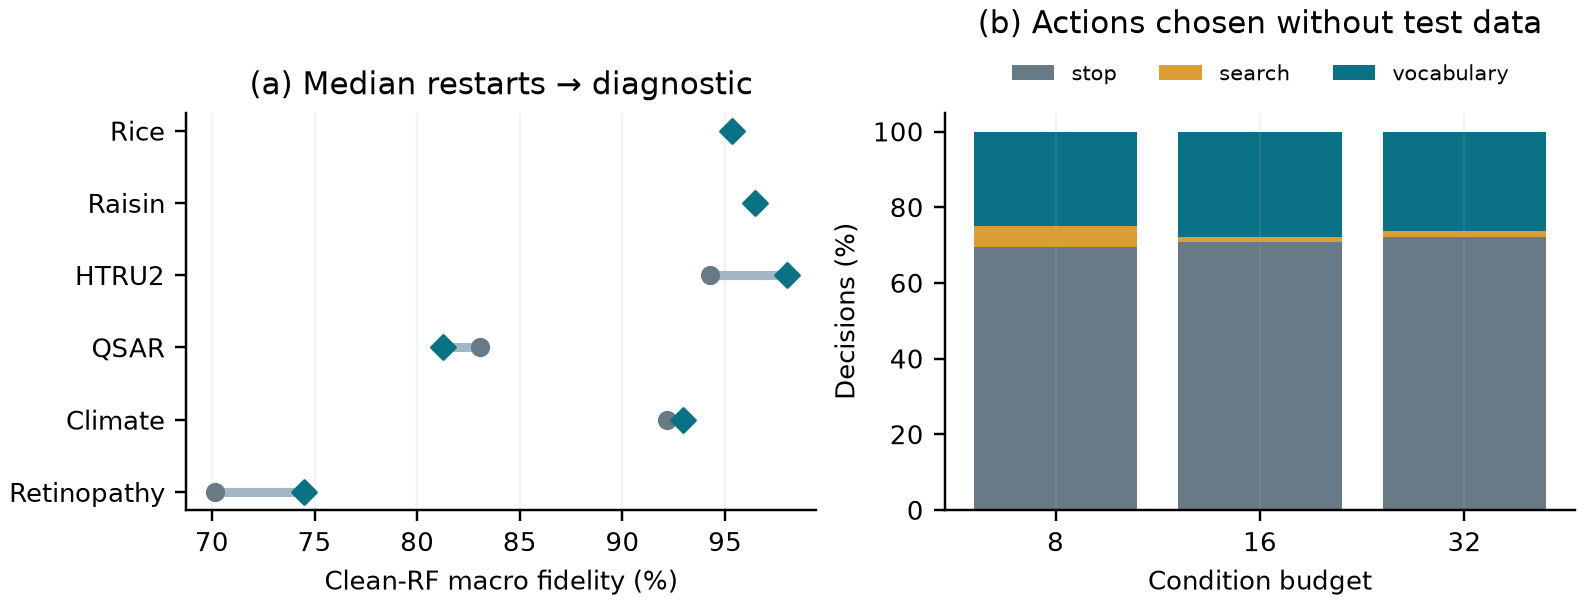
\includegraphics[width=\linewidth]{docs/research/major_revision_2026-10-15/independent_results.png}
\caption{Independent-cohort results. (a) Each segment compares median restarts (circle) and Diagnostic LFIO (diamond) on the clean-RF, eight-condition endpoint; points average the three splits within each dataset. (b) Controller actions use fitting-internal evidence only. CPU cost is reported separately in Table~\ref{tab:independent-main}.}
\label{fig:independent}
\end{kbfigure}
Absolute scoring avoids giving an enlarged vocabulary an automatically larger work allowance. Enumeration and score cost still vary, so CPU measurements remain necessary. The time accounting charges the controller's extra probes; an allocation policy that saves final scores can still lose wall time to pilot fitting and vocabulary construction. Conversely, the native tree's low CPU cost remains relevant even when a DNF policy closes a small fidelity gap. The secondary-budget and teacher/noise results are exported separately rather than selected after inspecting their test maxima.

\subsection{Real-task capacity and search intervals}\label{sec:certificate-results}
\begin{kbtable}
\centering
\caption{Real-task decomposition bounds for clean RF, seed 6001, eight conditions. All fitting rows and complete supported depth-two pools participate. Collision and capacity/search intervals are balanced-error percentage points; the final column counts proven-optimal head solves out of two, with a 15-second limit per head. Timeout dual bounds remain valid but do not certify an optimum. The MDL language nests all median predicates.}
\label{tab:real-certificates}
\small
\begin{adjustbox}{max width=\linewidth}
\begin{tabular}{lrrrrrrrr}
\toprule
Dataset & Vocabulary & $n_{fit}$ & $d_{pred}$ & Bodies & Collision & Capacity interval & Search interval & Optimal \\
\midrule
Rice & Median & 2286 & 7 & 98 & 7.27 & [0.09, 0.09] & [0.05, 0.05] & 2/2 \\
Rice & MDL & 2286 & 20 & 767 & 4.33 & [0.32, 1.43] & [0.00, 1.11] & 0/2 \\
Raisin & Median & 540 & 7 & 98 & 10.67 & [0.00, 0.00] & [0.18, 0.18] & 2/2 \\
Raisin & MDL & 540 & 20 & 734 & 5.91 & [0.24, 2.42] & [0.00, 2.18] & 0/2 \\
HTRU2 & Median & 10738 & 8 & 128 & 9.02 & [0.02, 0.02] & [0.07, 0.07] & 2/2 \\
HTRU2 & MDL & 10738 & 24 & 1082 & 4.22 & [0.00, 3.67] & [0.22, 3.89] & 0/2 \\
QSAR & Median & 634 & 41 & 3196 & 0.24 & [0.00, 17.73] & [0.00, 17.73] & 0/2 \\
QSAR & MDL & 634 & 86 & 14082 & 0.00 & [0.00, 14.69] & [0.00, 14.69] & 0/2 \\
Climate & Median & 324 & 18 & 648 & 0.00 & [0.31, 6.27] & [0.00, 5.96] & 0/2 \\
Climate & MDL & 324 & 22 & 963 & 0.00 & [0.22, 5.26] & [0.00, 5.04] & 0/2 \\
Retinopathy & Median & 691 & 19 & 648 & 20.56 & [0.16, 15.06] & [0.00, 14.91] & 0/2 \\
Retinopathy & MDL & 691 & 35 & 2149 & 12.96 & [0.00, 17.55] & [0.00, 17.55] & 0/2 \\
\bottomrule
\end{tabular}
\end{adjustbox}
\end{kbtable}

The 24 real-task head solves establish \IndependentOptimal{} optimality certificates; other solves retain available dual bounds and solver incumbents, using the decoder floor and feasible heuristic where solver bounds are unavailable. The intervals in Table~\ref{tab:real-certificates} implement Equation~\ref{eq:intervals} on all fitting rows, rather than relying on parity alone. A positive capacity lower bound certifies that no program in the specified pool at eight tests attains the unrestricted encoding floor. A positive search lower bound certifies an improvement over the chosen heuristic program by an executable solver incumbent. Wide intervals leave the mechanism unresolved.

The median languages of Rice, Raisin and HTRU2 illustrate a different situation from a high-dimensional unique encoding: repeated patterns give a positive collision floor, while the median-pool search shortfall can be small. Enrichment lowers that floor, but the resulting larger candidate class can make the same small description budget and finite search more restrictive. For QSAR and other sparse partitions a near-zero collision floor alone is weak evidence; the finite-budget oracle or held-out interventions are needed. Neither the sample decomposition nor a solver optimum guarantees a corresponding held-out improvement.

\subsection{Explicit generalization follow-up}\label{sec:generalization-results}
The separate extension uses the same six datasets, new seeds 7001--7003, both teachers and both noise levels. It refits the three DNF base learners at 8/16/32 conditions, giving 648 base/budget fits. The 20\% validation fold is divided by raw duplicate groups into approximately equal selection and calibration partitions; the overall allocation is about 60/10/10/20 for fitting/selection/calibration/test. Only the selection partition chooses the original model. Generalization paths use fitting data only, and calibration choices are persisted before test inference. This extension follows inspection of the earlier results and does not supply additional independent dataset units.

\begin{kbtable}
\centering
\caption{Explicit rule generalization on the six previously studied datasets with new seeds 7001--7003. Each row uses the same 648 base/budget fits (three learners, 72 teacher settings, three budgets). Reduction averages per-fit relative condition savings, counting zero-size originals as zero savings. Macro fidelity changes are paired with each original; descriptive intervals resample six dataset means. Boolean and semantic exact stages preserve global predictions. The two-point tolerance applies to two-class balanced error under the stated calibration assumptions, not a deterministic test-set guarantee.}
\label{tab:rule-generalization}
\small
\begin{adjustbox}{max width=\linewidth}
\begin{tabular}{lrrrrrrrr}
\toprule
Variant & Tests & Bodies & Features & Cuts & Saved (\%) & $\Delta$ fidelity (pp) & 95\% interval & Smaller /648 \\
\midrule
Original & 7.04 & 3.93 & 5.57 & 6.01 & 0.0 & +0.00 & [+0.00, +0.00] & 0 \\
Boolean exact & 7.04 & 3.93 & 5.57 & 6.01 & 0.0 & +0.00 & [+0.00, +0.00] & 0 \\
Semantic exact & 7.02 & 3.93 & 5.57 & 6.01 & 0.1 & +0.00 & [+0.00, +0.00] & 7 \\
Grow constrained & 5.70 & 3.68 & 4.90 & 5.19 & 18.9 & -0.26 & [-0.39, -0.10] & 365 \\
Empirical gate & 5.84 & 3.71 & 4.99 & 5.30 & 16.3 & -0.18 & [-0.28, -0.06] & 324 \\
Simultaneous bound & 6.64 & 3.85 & 5.43 & 5.79 & 4.8 & -0.02 & [-0.06, +0.01] & 103 \\
\bottomrule
\end{tabular}
\end{adjustbox}
\end{kbtable}

The numerical semantic exact stage reduces total conditions in 7 of 648 fits, with mean per-fit savings of 0.1\% [0.0, 0.2]. All exact-stage test predictions are unchanged, and global interval proofs are replayed. The grow-only path admits approximate candidates for 365 fits; the empirical and simultaneous-bound gates select a nonexact model in 323 and 99 fits, respectively. The simultaneous-bound variant saves 4.8\% of conditions with a paired test macro-fidelity change of -0.02 points [-0.06, +0.01]. These are repeated-split results on known datasets, not human-comprehension evidence or new external validation.

Boolean absorption/complement merging finds no additional reductions in these already-short programs. Numerical equivalence compression also has limited headroom. Approximate generalization provides most of the compression, and its empirical-only gate is less conservative than the simultaneous upper-bound gate. Neither a small mean fidelity change nor zero observed large losses establishes a distribution-free guarantee. Median incremental CPU for the shared generalization path and both gates is 0.0067 seconds per fit; this additional work is outside the original neighbor-scoring allowance and is reported separately.

\begin{kbtable}
\centering
\caption{Generalization effects by base learner, across 216 fits each. The numerical semantic stage uses threshold implications that a Boolean-only simplifier cannot exploit.}
\label{tab:generalization-base}
\small
\begin{adjustbox}{max width=\linewidth}
\begin{tabular}{lrrrrr}
\toprule
Base & Stage & Original tests & Final tests & Saved (\%) & $\Delta$ fidelity (pp) \\
\midrule
DiagnosticLFIO & Boolean exact & 7.09 & 7.09 & 0.0 & +0.00 \\
DiagnosticLFIO & Semantic exact & 7.09 & 7.07 & 0.2 & +0.00 \\
DiagnosticLFIO & Simultaneous bound & 7.09 & 6.57 & 6.2 & -0.03 \\
MedianRestarts & Boolean exact & 6.96 & 6.96 & 0.0 & +0.00 \\
MedianRestarts & Semantic exact & 6.96 & 6.96 & 0.0 & +0.00 \\
MedianRestarts & Simultaneous bound & 6.96 & 6.69 & 3.1 & +0.03 \\
MDLRestarts & Boolean exact & 7.06 & 7.06 & 0.0 & +0.00 \\
MDLRestarts & Semantic exact & 7.06 & 7.04 & 0.2 & +0.00 \\
MDLRestarts & Simultaneous bound & 7.06 & 6.67 & 5.1 & -0.05 \\
\bottomrule
\end{tabular}
\end{adjustbox}
\end{kbtable}


\subsection{Predictions without specified features}\label{sec:forgetting-results}
This post hoc extension reuses the preceding 648 source fits and applies forgetting separately to Original and BoundedGeneralize, giving 1,296 source programs. It introduces no new teacher fitting, splits or independent dataset units. We compile every active singleton, a separately counted unused-feature identity control, and the joint pairs needed by two policies. Fixed queries use the lowest active indices. Selection queries maximize certified coverage on selection inputs; ties prefer fewer combined tests/bodies and then lower indices. The two-feature policy adds a second coordinate to the selected singleton. All formulas, missing-coordinate choices and fitting medians are saved before test inference. Pair results exclude programs with fewer than two active features.

\begin{kbtable}
\centering
\caption{Feature forgetting on the existing 648 fits, applied to Original and BoundedGeneralize separately. Fixed uses the lowest active indices; Selection maximizes certified coverage on selection inputs only. Two-feature rows require at least two active coordinates. Coverage is averaged equally over six datasets. Exact reports completed universal compilations; other cases use a conservative lower bound. L/U tests average both explicit formulas; Grow is the fraction whose combined count exceeds the source count. Fill disagrees with the fully observed source after fitting-median imputation; it is a forced prediction reference with a different coverage denominator. All certificates concern the source surrogate.}
\label{tab:feature-forgetting}
\small
\begin{adjustbox}{max width=\linewidth}
\begin{tabular}{lllrrrrrr}
\toprule
Source & Missing & Policy & Fits & Certified (\%) & Exact (\%) & L/U tests & Grow (\%) & Fill disagree (\%) \\
\midrule
Original & 1 & Fixed & 648 & 61.0 & 98.5 & 109.47 & 73.0 & 16.39 \\
Original & 1 & Selection & 648 & 80.8 & 98.6 & 123.08 & 72.2 & 9.74 \\
Original & 2 & Fixed & 610 & 36.0 & 98.4 & 83.70 & 56.4 & 19.98 \\
Original & 2 & Selection & 610 & 61.4 & 98.7 & 108.49 & 61.6 & 11.96 \\
Bounded & 1 & Fixed & 648 & 59.2 & 98.5 & 106.68 & 72.7 & 16.96 \\
Bounded & 1 & Selection & 648 & 79.5 & 98.6 & 119.38 & 70.7 & 10.36 \\
Bounded & 2 & Fixed & 607 & 35.3 & 98.4 & 82.89 & 56.0 & 20.53 \\
Bounded & 2 & Selection & 607 & 59.3 & 98.7 & 107.36 & 59.6 & 12.82 \\
\bottomrule
\end{tabular}
\end{adjustbox}
\end{kbtable}

For Original, selection-based single-feature forgetting certifies 80.8\% of test inputs, with a descriptive dataset-cluster interval of [74.0, 87.2], and a paired coverage gain of +19.8 points [+12.7, +26.9] over the fixed-index query. The nested two-feature policy certifies 61.4\% on 610 eligible programs. For the singleton selection policy, coverage conditional on the source head and default classes is 77.3\% and 80.8\%, respectively (using only nonempty class subsets). All 7,551,125 recorded assigned test queries agree with their respective source programs. The independent checker replays 16,187,153 selection/test retained-row queries across 14,834 compiled queries. 752 compilations exhaust a fixed resource limit and are marked conservative. The singleton selection policy has a larger combined representation than its source in 72.2\% of fits; the median and maximum combined condition counts are 21 and 4,379. The extension therefore establishes partial-input certificates, not uniformly shorter descriptions. These repeated uses of the same rows are implementation checks, not independent statistical observations.

\begin{kbfigure}
\centering
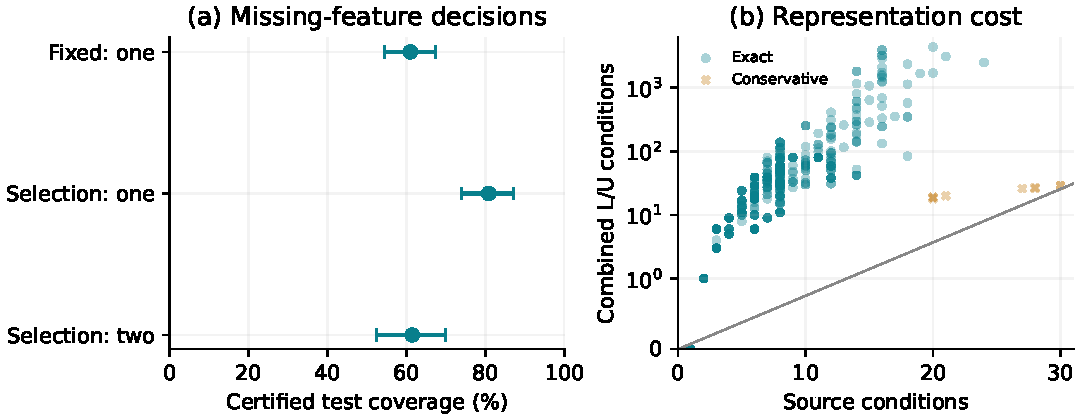
\includegraphics[width=\linewidth]{docs/research/feature_forgetting_2026-10-16/forgetting.pdf}
\caption{Partial-input certificates and representation cost for Original. Left: dataset-equal coverage with descriptive six-dataset cluster intervals; two-feature coverage uses eligible programs. Right: conditions in both compiled formulas versus the source program; the diagonal marks equal counts and the vertical axis uses a logarithmic scale above one. Larger representation cost is possible despite eliminating a feature.}
\label{fig:feature-forgetting}
\end{kbfigure}

The independent checker enumerates all forgotten-coordinate threshold cells for each recorded selection/test retained row, without using the compiler's complement algorithm. It also replays choices and saved vectors. A source prediction after fitting-median imputation and the existential-only forced classifier provide references that always predict; their full-coverage errors have a different denominator from our selective predictions. Zero observed source contradictions supports the implementation check, while completion-invariant assignment follows from the constructed envelope. Neither source agreement nor abstention supplies teacher-level certification. No minimum explanation or measured human-comprehension result is inferred.

Different base vocabularies and model sizes leave different room for simplification. Feature counts, threshold counts and canonical short-circuit checks accompany the exported results. They describe executable structure and do not substitute for human prediction-simulation or error-detection experiments. The experiment's grouped, fixed-benchmark sampling is reported alongside the iid assumptions needed for the binomial guarantee.

\subsection{Constrained, cost-aware and residual-query extension}\label{sec:contextual-results}
This exploratory extension fixes its code and protocol before evaluation and reuses the 648 Original source programs above. It adds no training, new datasets or independent replication. For each program, five greedy policies select hidden active coordinates at selection coverage requirements $q\in\{0.7,0.8,0.9\}$. Uniform costs and controlled heterogeneous costs $c_j=1+(j\bmod5)$ give 19,440 policy/target/profile records. Every candidate, score and final choice is saved before indexing the test matrix. The primary descriptive endpoint compares CostAware with Coverage at $q=0.8$ under heterogeneous costs. Both policies enforce the same selection requirement and resource limits. Costs depend only on declared coordinate indices; they are sensitivity scenarios rather than application acquisition measurements.

\begin{kbtable}
\caption{Cost-constrained hiding on 648 Original programs. Heterogeneous controlled costs, selection coverage requirement $q=0.8$; means weight the six datasets equally and include empty-subset fallbacks. Hidden cost is a fraction of total active-feature cost.}
\label{tab:contextual-cost}
\centering\small
\begin{tabular}{lrrr}
\toprule
Policy & Hidden cost (\%) & Features & Test coverage (\%)\\
\midrule
Fixed & 23.4 & 1.44 & 89.1\\
Frequency & 23.4 & 1.43 & 89.1\\
Impact & 26.1 & 1.54 & 90.1\\
Coverage & 25.9 & 1.54 & 90.0\\
CostAware & 27.9 & 1.54 & 89.9\\
\bottomrule
\end{tabular}
\end{kbtable}

CostAware hides 27.9\% of active-coordinate cost versus 25.9\% for Coverage, a paired difference of 2.0 points (descriptive dataset-cluster interval [0.9,3.1]). Test certified coverage is 89.9\%; the selection constraint does not guarantee the test target, which is missed by 9.7\% of fits. Empty hiding sets occur in 22.2\% of fits. These controlled coordinate costs are not measured acquisition or privacy costs.

Across 7,507 previous Original projections, residual queries encounter 0 unresolved projections and add 51,892 assigned test-row queries relative to the bounded compiler, with 0 lost assignments. These are repeated evaluation events, not independent observations. On the 32 deliberately large compiled representations (3837--5260 combined tests), median Python allocation peaks are 1528.7 KiB for compilation and 10.8 KiB for queries. Median setup-plus-first-batch CPU is 0.4478 versus 0.0012 seconds; warm-batch CPU is 0.00629 versus 0.00088 seconds. CPU uses three fresh repetitions without tracing, separately from allocation measurement. The batch contains at most 64 test rows. Python peaks omit native allocations, and this stress subset does not establish a general speed advantage.

All candidate coverage values, final decisions and test vectors are replayed. Small candidate subsets are independently checked by threshold-cell enumeration; the audit records subsets exceeding its enumeration cap separately. The query engine is also checked on the previous Original singleton/pair/control projections. Logical success concerns the source surrogate under the stated completion domain. Selection coverage supplies no statistical lower bound on deployment coverage, and the greedy paths need not maximize hidden cost globally.

\begin{kbfigure}
\centering
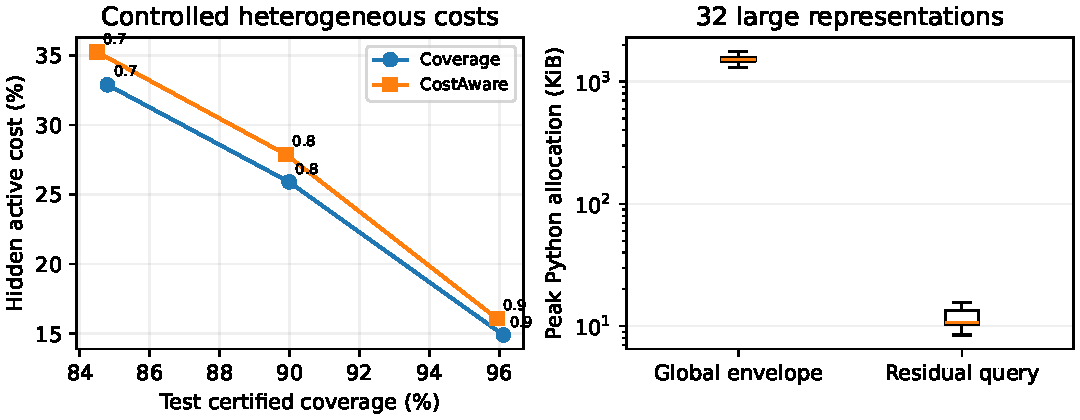
\includegraphics[width=\linewidth]{docs/research/contextual_forgetting_2026-10-16/contextual.pdf}
\caption{Cost selection and residual representation. Left: dataset-equal test coverage versus hidden active cost at selection requirements 0.7, 0.8 and 0.9 (point labels). Right: Python allocation peaks on 32 deliberately large compiled representations, with logarithmic scale. CPU is measured separately without allocation tracing. Cache entries and allocation bytes do not measure human understanding.}
\label{fig:contextual-forgetting}
\end{kbfigure}

Background constraints are evaluated separately on controlled tasks with a known construction. For $F=(x>0)$, hidden $x$, retained $y\in\{-2,-1,0,1,2\}$ and true domain $x=y$, unrestricted queries certify no rows. Supplying the equality certifies all five, including both classes; supplying only $x\geq y$ certifies two, and the band $y-1/4<x\leq y+1/4$ certifies four. Adding $y\leq1$ to equality correctly rejects the retained input $y=2$ as infeasible. Supplying the wrong equality $x=y-2$ certifies all five under that assumption but disagrees with the true domain on two. This negative control makes the conditional scope of a background certificate observable. An independent checker enumerates threshold cells and uses exact Fourier--Motzkin elimination on 900 additional queries from 100 random three-coordinate systems, rather than the engine's difference-graph procedure. These controls validate supported constraint semantics; they do not demonstrate gains on real tasks with verified domain constraints.

\subsection{What the development evidence does and does not add}\label{sec:development}
The supplement retains the original ten-dataset studies, including breast cancer, banknote, ionosphere, spambase, red wine, grid stability, MAGIC, Haberman, Sonar and transfusion~\citep{magic,haberman,sonar,transfusion}. Their validation-opportunity and scored-work controls informed the new policy. Under matched scored work the clean repair-minus-restarts fidelity difference was $-0.10$ points, interval $[-1.14,1.04]$, and the noisy difference was $+0.30$ points, interval $[-0.31,1.47]$. These results do not justify making repair the default additional investment. The original four-budget full grid also cost a median 8.35 seconds versus 0.61 seconds without both added components, motivating an explicit absolute allowance.

The older five-bit oracle and parity construction retain their mechanistic purpose: they demonstrate that local search can fail within a feasible language and that description capacity can exclude a concept. The retrospective vocabulary analysis replays 120 native-teacher settings and 960 saved validation/test predictions, distinguishing unrestricted encoding ceilings from feasible small-model performance. These are development and retrospective analyses, not new independent replications. No such observation is pooled with the independent six-dataset endpoint or used to relabel an inconclusive primary comparison as confirmed.

\section{Discussion and limitations}
The practical contribution is an auditable way to distinguish a mechanism, a certificate and an action witness. Conflicting encodings give an exact sample-level obstruction for every deterministic decoder. Finite-pool solver bounds can certify additional description or search loss. Fitting-only held-out interventions can guide an action without claiming such a certificate. Their conclusions have different scopes and should not be collapsed into a single diagnosis of test error.

The algorithmic primitives are established. The absolute-budget search adapts the earlier restart implementation; MDL discretization, greedy repair, and pilot selection are not new in isolation. The controller and integrated attribution experiment are the concrete contribution. The primary fidelity comparison remains limited by six dataset units, conservative pilot selection, and the stronger fixed MDL and direct baselines. The observed resource use is not a fidelity noninferiority result. A larger independent collection could test whether learned allocation rules or more reliable internal probes improve this tradeoff, but the current protocol is not retuned to obtain that result.

No capacity witness fires in the 216 real-data budget decisions, even though some fitting-pool capacity lower bounds are positive. The pilot uses different observations, finite search and a one-percentage-point gain threshold; it is not validated here as a sensitive detector of every certified capacity restriction. A constructed XOR check verifies that the larger-budget probe can fire while deployment remains within the original budget, but this positive control does not supply real-task generalization evidence.

The oracle is complete only for its supplied supported depth-two pool and fixed body/condition caps. Timeouts can leave broad intervals, and matrix construction is itself costly. The partition floor can become vacuous when observations are nearly unique; no population calibration or uncertainty guarantee is derived from it. The controller's capacity witness changes the permitted model size, but finite search and pilot selection prevent it from certifying an irreducible capacity barrier. It recommends no automatic increase in the deployment budget.

The six new datasets are a modest, intentionally selected tabular collection; Rice and Raisin share a domain. Repeated splits overlap, corruptions are synthetic, and no natural label errors, temporal shifts, naturally missing inputs or active teacher queries are tested. Hard teacher labels discard uncertainty. The two teacher families improve boundary diversity without guaranteeing strong reference-label performance on every task. Their teacher-quality measurements constrain any downstream accuracy claim.

The condition count is explicit but not a universal measure of interpretability. Ordered intervals, multi-value rule sets, native trees and single-head conjunctions have different semantics and effective capacity. Charging each atomic test prevents free interval or multi-value compression, but can differ from a comparator's preferred native metric. BRCG-light is approximate; FastSRS uses a documented initialization override and a fixed regularization grid; NeuRules uses a fixed training recipe and six sizes. MOSS, exact branch-and-price, oblique rule boosting, FI-rules4XAI and CORTEX remain related methods rather than executed numerical comparators~\citep{liu2025moss,behzadimanesh2026,kozielski2025,kopanja2025}. No human-subject or causal-faithfulness claim follows from executable size or prediction agreement. Explicit generalization preserves a certified relation to the original surrogate, while approximate coverage expansion requires a separate statistical assumption and can reject all shorter candidates when calibration support is small. Its operators and confidence limits are classical; the extension does not establish globally minimum descriptions or better human understanding. Feature forgetting adds deterministic partial-input certificates for a selected source surrogate. Unrestricted completions can lie off the data manifold, while background-constrained certificates are only as applicable as the supplied constraints. The exact implementation supports difference bounds rather than arbitrary domain theories, and verified real-data constraints remain unevaluated. Global formulas can grow; residual queries reduce expansion but have their own search/cache limits and do not supply readable global explanations. Cost-aware hiding uses synthetic coordinate costs and a greedy search, and maximizing selection coverage proves neither deployment coverage nor minimal explanatory features.

\section{Conclusion}
A compact surrogate's disagreement with its teacher can reflect information discarded by its predicates, limits of its feasible program class, or search shortfall. The revised framework puts these restrictions on a common empirical scale with valid finite-pool bounds, and Diagnostic LFIO tests a fitting-only effort-allocation loop under explicit condition and scoring budgets. Independent numerical-teacher experiments and recent direct baselines support a qualified result: the diagnostics are executable and informative in defined cases, while adaptive allocation does not establish a general advantage over fixed enriched predicates. The explicit-generalization extension adds verified numerical compression and calibrated coverage expansion, yielding modest structural savings with small measured fidelity changes on new splits of the same tasks. Numerical feature forgetting then exposes which decisions remain invariant when specified coordinates are unknown. Exact difference constraints, explicit infeasibility, bounded residual queries and coverage-constrained cost selection extend this source-relative guarantee to a defined partial-input task. The controlled cost improvement and recovery from compiler fallbacks motivate broader tests with measured feature costs and verified domain knowledge. The release preserves replayable decisions, failures, teacher quality and computational cost.

\appendix
\section{Data provenance and reproduction}\label{app:extension}
The dataset registry is \path{data/research/prospective_2026-10-15/sources.json}. Its six source records link directly to the UCI pages for datasets 545, 850, 372, 254, 252 and 329. Original downloaded archives and SHA-256 hashes are retained. All are identified under the repository's CC BY 4.0 license. The source files, feature exclusions and positive classes are defined by \path{run_prospective_revision.py}. The prospective protocol is \path{docs/research/MAJOR_REVISION_PROTOCOL_2026-10-15.md}; it predates all new model fits. The protocol was frozen on 15 October UTC and the revision continued on 16 October China Standard Time.

Execution uses \path{run_prospective_revision.py}; real-task bounds use \path{certify_real_revision.py}; independent replay and aggregation use \path{generate_major_revision.py}. The audit checks 72 settings, 576 method grids and 1,728 budget selections, including infeasibility, and reruns all 216 controller decisions from fitting data. The output records include per-dataset results, all secondary endpoints, warnings, versions, source hashes, leave-one-dataset sensitivity and dataset-cluster intervals. Official FastSRS provenance and its MIT license accompany the code; upstream NeuRules files are pinned separately. No native baseline implementation is renamed as a home-written approximation. The explicit-generalization protocol and implementation are documented in \path{docs/research/RULE_GENERALIZATION_PROTOCOL_2026-10-16.md} and \path{docs/research/RULE_GENERALIZATION_2026-10-16.md}; executable records and audits are in the corresponding dated result and report directories. Feature-forgetting execution and independent projection checks use \path{run_feature_forgetting.py} and \path{generate_feature_forgetting.py}; its separate protocol fixes source programs, missing-coordinate policies, representation counts and failure limits. The contextual/cost extension uses \path{run_contextual_forgetting.py} and \path{generate_contextual_forgetting.py}, with its separate frozen protocol, independent Fourier--Motzkin checker and 19,440 policy records. The earlier solver certificates concern their original samples and are not relabeled as certificates for the new splits.

\section{Supplementary capacity controls}\label{app:synthetic}
For $d$-bit parity every pure positive conjunction must fix all $d$ bits, and exactly $2^{d-1}$ positive assignments exist. Thus a single-head DNF for exact parity needs $2^{d-1}$ full-depth bodies and $d2^{d-1}$ tests. Complementing the head does not remove the requirement. This elementary capacity example belongs to the development supplement; it does not establish that a real-data loss is caused by capacity. The real-task intervals address that question for the evaluated finite pools.

The earlier replacement identity computes union coverage after deleting an incumbent body, so a replacement can retract false-positive head coverage that additions cannot remove. It explains a move's mechanism without guaranteeing global optimization or better generalization. Both identities and the older exact generated tasks remain separately reproducible; the independent conclusions do not depend on treating them as novel generalization theorems.

\section*{Data and code availability}
The current release includes a source package, a reproducibility-code package and experiment records under \path{docs/research/contextual_forgetting_2026-10-16/}. Its contextual/cost-query records are in \path{results/contextual_forgetting_20261016/}; it also retains the frozen allocation, generalization and global feature-forgetting cohorts. The preceding global feature-forgetting release remains under \path{docs/research/feature_forgetting_2026-10-16/}; the earlier generalization and allocation snapshots remain under their own dated directories. The experiment archive contains fitting/selection/calibration/test partitions, hard teacher outputs, model exports, saved choices, test prediction vectors, timing, source/data locks, solver bounds, controlled constraint queries and separate untraced CPU measurements. Earlier snapshots retain their original identities. The current version and package names are listed in \path{docs/research/CURRENT_RELEASE.md}; commands and package checks are documented in \path{docs/research/REPRODUCE.md}. The separate \texttt{LFIO\_Development\_Supplement.pdf} preserves the chronological development evidence.

\section*{Funding}
This research was supported by Zhejiang Provincial Natural Science Foundation
of China under Grant No. LQN26F020019.

\section*{CRediT authorship contribution statement}
\textbf{Xu Wang:} Conceptualization, Methodology, Software, Investigation,
Validation, Writing -- original draft, Writing -- review \& editing.
\textbf{Zhiqiang Chen:} Writing -- original draft, Writing -- review \& editing,
Investigation (literature collection).

\section*{Declaration of generative AI and AI-assisted technologies}
OpenAI Codex and DeepSeek assisted methodological discussion, code development, manuscript revision and literature checking. Reported numerical results were produced by the accompanying executable experiment and analysis scripts. The authors remain responsible for the scientific content and final interpretation.

% Author-supplied competing-interest declarations
% can be added here before submission.
\bibliographystyle{elsarticle-num}
\bibliography{references}
\end{document}
